\graphicspath{ {images/2_source_localization/} }
\chapter{Sound Source Localization}
\section{Sound Source Localization Methods}
Sound Source Localization (SSL) \todo{Abbr Verzwichnis} is a well researched area with many applications.

The basic system can be brought into two categories, time based or power based methods.
\subsection{Power based SSL}
The idea of power based SSL is based of the known propagation properties of sound waves in air.
BlaBlaBla \todo{short text}
However for this method to work some properties of the sound source have to be known.
Additionaly the sensors that measure the sound power levels have to be calibrated \dots 

\subsection{Time Based SSl}



\begin{figure}
    \centering
    \begin{subfigure}[b]{0.45\textwidth}
        \centering
        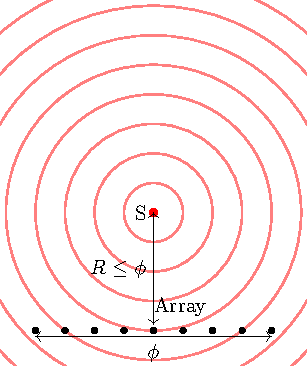
\includegraphics[width=\textwidth]{NearField.pdf}
        \caption{Near-Field Case}
        \label{fig:y equals x}
    \end{subfigure}
    \hfill
    \begin{subfigure}[b]{0.45\textwidth}
        \centering
        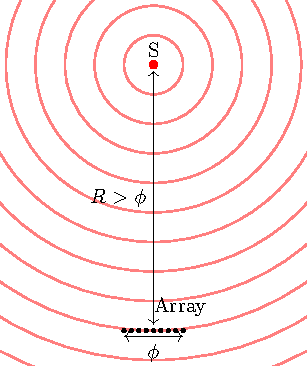
\includegraphics[width=\textwidth]{FarField.pdf}
        \caption{Far-field Case}
        \label{fig:three sin x}
    \end{subfigure}
    \caption{Three simple graphs}
    \label{fig:three graphs}
\end{figure}



%\begin{figure}
%    \centering
%%    \includegraphics[width=0.25\textwidth]{mesh}
%    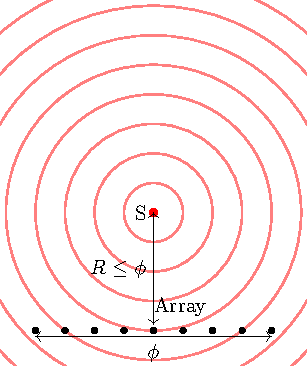
\includegraphics[]{NearField.pdf}
%    \caption{a nice plot}
%    \label{fig:mesh1}
%\end{figure}
